% IEEE QCE 2026 poster -- A0 portrait, 3 columns.
% Content distilled from main.tex (final, 100-instance numbers).
% Compile with pdflatex (twice). Figure: figures/fig_sa_vs_qpu.pdf
\PassOptionsToPackage{table}{xcolor} % enable \rowcolor (beamer loads xcolor itself)
\documentclass[final]{beamer}
\usepackage[scale=1.29,size=a0,orientation=portrait]{beamerposter}
\usepackage[utf8]{inputenc}
\usepackage[T1]{fontenc}
\usepackage{lmodern}
\usepackage{amsmath,amssymb}
\usepackage{booktabs}
\usepackage{array}
\usepackage{graphicx}
\usepackage{tikz}
\usepackage{xcolor}
\usepackage{colortbl} % defines \rowcolor (pgf/xxcolor swallows xcolor's table option)
\usepackage{ragged2e}

%==================== colours ====================
\definecolor{deepblue}{RGB}{15,42,78}     % title bar, block headers
\definecolor{midblue}{RGB}{23,84,130}     % sub-emphasis
\definecolor{saBlue}{RGB}{31,119,180}     % SA  (matches figure)
\definecolor{qpuRed}{RGB}{200,30,38}      % QPU (matches figure)
\definecolor{accent}{RGB}{222,106,38}     % the peak
\definecolor{blockbg}{RGB}{245,247,250}
\definecolor{bandgray}{RGB}{234,239,244}
\definecolor{accentlight}{RGB}{171,201,232}
\definecolor{ink}{RGB}{26,26,26}

%==================== block / font theme ====================
\setbeamercolor{block title}{fg=white,bg=deepblue}
\setbeamercolor{block body}{fg=ink,bg=blockbg}
\setbeamercolor{block alerted title}{fg=white,bg=qpuRed}
\setbeamercolor{block alerted body}{fg=ink,bg=blockbg}
\setbeamerfont{block title}{size=\large,series=\bfseries}

% custom blocks with generous inner padding so text never touches the border
\setbeamertemplate{block begin}{
  \par\vskip0.5cm
  \begin{beamercolorbox}[sep=0.42cm,rounded=true,shadow=true]{block title}
    \usebeamerfont*{block title}\hspace{0.25cm}\insertblocktitle
  \end{beamercolorbox}
  \vskip-0.08cm
  \usebeamerfont{block body}
  \begin{beamercolorbox}[sep=0.55cm,vmode,rounded=true,shadow=true]{block body}
    \setlength{\leftskip}{0.45cm}\setlength{\rightskip}{0.6cm}\RaggedRight
}
\setbeamertemplate{block end}{
  \end{beamercolorbox}\vskip0.45cm
}
\setbeamertemplate{block alerted begin}{
  \par\vskip0.5cm
  \begin{beamercolorbox}[sep=0.42cm,rounded=true,shadow=true]{block alerted title}
    \usebeamerfont*{block title}\hspace{0.25cm}\insertblocktitle
  \end{beamercolorbox}
  \vskip-0.08cm
  \usebeamerfont{block body}
  \begin{beamercolorbox}[sep=0.55cm,vmode,rounded=true,shadow=true]{block alerted body}
    \setlength{\leftskip}{0.45cm}\setlength{\rightskip}{0.6cm}\RaggedRight
}
\setbeamertemplate{block alerted end}{
  \end{beamercolorbox}\vskip0.45cm
}
\setbeamertemplate{itemize item}{\color{deepblue}\raisebox{0.15ex}{\footnotesize$\blacktriangleright$}}
\setbeamertemplate{itemize subitem}{\color{midblue}\textbullet}
\setbeamertemplate{navigation symbols}{}
\setbeamercolor{itemize item}{fg=deepblue}
\setbeamercolor{structure}{fg=deepblue}

% list spacing: wide left margin so item labels (incl. wide markers) stay inside the block
\setlength{\leftmargini}{2.9em}
\setlength{\labelsep}{0.5em}
\setbeamertemplate{itemize/enumerate body begin}{\RaggedRight}
% "therefore/implies" marker, same size/baseline as the bullet so it does not overhang
\newcommand{\cimp}{\item[{\color{deepblue}\raisebox{0.12ex}{\footnotesize$\Rightarrow$}}]}

%==================== emphasis macros ====================
\newcommand{\hl}[1]{{\color{accent}\textbf{#1}}}      % the peak / key number
\newcommand{\sacol}[1]{{\color{saBlue}\textbf{#1}}}
\newcommand{\qpucol}[1]{{\color{qpuRed}\textbf{#1}}}
\newcommand{\lab}[1]{{\color{deepblue}\textbf{#1}}}    % inline sub-labels
\newcommand{\xstar}{x^{\star}}
% reading-order badge for block titles (white disc, dark number).
% \smash so the disc does not add height to the title bar; raise to centre on the title text.
\newcommand{\bnum}[1]{\smash{\raisebox{-0.27cm}{\tikz\node[circle,fill=white,text=deepblue,inner sep=1pt,minimum size=0.82cm,font=\normalsize\bfseries]{#1};}}\hspace{0.2cm}}

%==================== column lengths ====================
\newlength{\sepwid}\newlength{\onecolwid}\newlength{\fullwid}
\setlength{\sepwid}{0.022\paperwidth}
\setlength{\onecolwid}{0.298\paperwidth}
\setlength{\fullwid}{0.940\paperwidth}
\setlength{\topmargin}{-0.5in}

%==================== custom headline (band auto-sizes to content) ====================
\setbeamercolor{headbar}{bg=deepblue,fg=white}
\setbeamercolor{accentbar}{bg=accent}
\setbeamertemplate{headline}{
  \leavevmode
  % full-bleed band behind the header: overshoot all edges so the colour bleeds
  % off the page (no hairline slivers at the exact page boundary in any viewer)
  \begin{tikzpicture}[remember picture, overlay]
    \fill[deepblue] ([shift={(-1cm,1cm)}]current page.north west)
      rectangle ([shift={(1cm,-16.2cm)}]current page.north east);
  \end{tikzpicture}
  \begin{beamercolorbox}[wd=\paperwidth,sep=0pt]{headbar}
    \vskip1.6cm
    \begin{center}
      {\fontsize{72}{82}\selectfont\bfseries
        Difficulty Analysis of Posiform-Planted QUBO\par}
      \vskip0.35cm
      {\fontsize{72}{82}\selectfont\bfseries
        Benchmarks via Energy and Hamming Metrics\par}
      \vskip0.8cm
      {\fontsize{40}{46}\selectfont
        Yideun Kim \quad\textbullet\quad Dongjae Lee\par}
      \vskip0.28cm
      {\fontsize{31}{38}\selectfont\color{accentlight}
        Kangwon National University, Chuncheon, Republic of Korea
        \quad\textbullet\quad \texttt{rladlems1031@kangwon.ac.kr}\par}
      \vskip0.28cm
      {\fontsize{29}{36}\selectfont\color{accentlight}\itshape
        IEEE Int.\ Conf.\ on Quantum Computing and Engineering (QCE) 2026 --- Poster\par}
    \end{center}
    \vskip1.0cm
  \end{beamercolorbox}
  \begin{beamercolorbox}[wd=\paperwidth,ht=0.35cm,sep=0pt]{accentbar}\end{beamercolorbox}
  % KNU logo on a white badge, top-left, drawn on top of the band
  \begin{tikzpicture}[remember picture, overlay]
    \node[anchor=north west, fill=white, rounded corners=16pt, inner sep=11pt]
      at ([xshift=1.4cm, yshift=-0.95cm]current page.north west)
      {
\includegraphics[height=5.8cm]{figures/knu_logo.png}};
  \end{tikzpicture}
}

\setbeamercolor{footbar}{bg=deepblue,fg=white}
% footline left empty on purpose: beamerposter does not reserve footline space,
% so the footer bar is placed in-body after the conclusion (see end of frame).
\setbeamertemplate{footline}{}

\begin{document}
\begin{frame}[t]
\vskip0.4cm
\begin{columns}[t]

%==================================================== COLUMN 1
\begin{column}{\sepwid}\end{column}
\begin{column}{\onecolwid}

\begin{block}{\bnum{1}Motivation: the $0\%$-success wall}
\RaggedRight
Benchmarking QUBO solvers needs instances whose optimum is known yet that stay hard. \textbf{Posiform planting} gives a unique planted optimum~$\xstar$. A hardened variant adds random discrete-coefficient spin-glass QUBOs $R_i$ and scales the planted posiform $P$ by a coefficient $\alpha$:
\vskip0.4cm
\begin{center}\large
$\displaystyle Q_{\alpha}(x) \;=\; \sum_{i} R_i(x) \;+\; \alpha\,P(x)$
\end{center}
\vskip0.4cm
\begin{itemize}
  \item Hardness is graded by the \textbf{ground-state success rate} (success $=$ the exact planted $\xstar$, not merely ground-state energy).
  \item But across the whole hard regime that rate is \hl{identically $0\%$}.
  \cimp It \textbf{cannot rank} instances, solvers, or $\alpha$ within the hard regime. The benchmark loses its purpose.
\end{itemize}
\end{block}

\begin{block}{\bnum{2}Idea: measure the failures}
\RaggedRight
Instead of asking whether a run succeeded, we ask how close the failing runs come to $\xstar$. We use two quantities, over \textbf{failures only}, on a \textbf{fixed set of the $100$ hardest} instances:
\begin{itemize}
  \item \sacol{Energy gap} $\Delta E = E(x)-E(\xstar)\ge 0$ --- depth of the trap.
  \item \qpucol{Hamming distance} $\mathrm{HD}(x,\xstar)$ --- bit-distance to the answer.
\end{itemize}
\vskip0.3cm
These turn the flat $0\%$ into a \textbf{continuous, rankable difficulty curve}. Neither quantity is new --- the \textbf{contribution is the protocol}: failure-conditioning on a fixed hardest set, cross-checked on real hardware.
\end{block}

\begin{block}{\bnum{3}Methodology}
\RaggedRight
\lab{Instances.} $500$ posiform-planted QUBOs on the D-Wave \textbf{Pegasus P16} graph ($n{=}5612$ qubits), \texttt{lin2} coefficients $R_{ij}\!\in\!\{-1,+1\}$. Kernighan--Lin bisection into $\le 16$-qubit blocks, each $R_i$ solved exactly; $\xstar=$ concatenated block ground states (global min of $\sum_i R_i$); $P=$ posiform of a planted 2-SAT with unique solution~$\xstar$.
\vskip0.35cm
\lab{Fixed set.} Rank instances by total SA failing-reads across the sweep. Fix the hardest $100$, \textbf{chosen from SA alone, before any QPU run}, so the cross-solver agreement is not circular.
\vskip0.35cm
\lab{Metrics.} \texttt{lin2} $\Rightarrow$ integer $R$ energies $\Rightarrow$ report $\Delta E$ in units of the minimal $R$-gap $\Delta_R{=}1$ (comparable across instances). All statistics are \textbf{conditional on failure} ($x\neq\xstar$).
\vskip0.35cm
\lab{Protocol.} \texttt{neal} SA package, $1000$ sweeps, $100$ reads / (instance,\,$\alpha$). Cross-check: same $100$ instances on a \textbf{D-Wave Advantage} annealer --- hardware-native, auto-scale, two-gauge, $100$ reads $\times\,20\,\mu$s.
\end{block}

\end{column}

%==================================================== COLUMN 2
\begin{column}{\sepwid}\end{column}
\begin{column}{\onecolwid}

\begin{block}{\bnum{4}Why report both metrics}
\RaggedRight
\lab{At $\alpha{=}0$ ($R$ alone, degenerate):}
\begin{itemize}
  \item \hl{$56.1\%$} of samples reach an $R$ ground state ($\Delta E{=}0$)\dots
  \item \dots yet \hl{$0\%$} equal $\xstar$, and HD is maximal ($459=8.2\%$ of $n$).
  \cimp $\Delta E$ alone reads as \textbf{solved}, yet only \textbf{HD} reveals that no sample is near $\xstar$.
\end{itemize}
\vskip0.35cm
\lab{As $\alpha$ grows:}
\begin{itemize}
  \item HD \sacol{decreases} (failures move closer in bits to $\xstar$)\dots
  \item \dots while $\Delta E$ rises to a \hl{peak} (failures get deeper in energy).
  \cimp \textbf{Opposite trends on the same samples} --- each metric captures what the other misses.
\end{itemize}
\end{block}

\begin{block}{\bnum{5}The $\Delta_R$ floor and the $\alpha P$ peak}
\RaggedRight
Failure-conditioned $\Delta E$ traces $\Delta E = \Delta R + \alpha\,\Delta P$ directly:
\begin{itemize}
  \item \lab{Floor.} For $\alpha\in[10^{-9},10^{-4}]$, $\Delta E$ is flat at the bare $R$-trap depth --- mean $1.10$, median exactly $1$ (one $\Delta_R$); $\alpha\Delta P$ negligible. HD flat $\approx 73$.
  \item \lab{Peak.} Past $\alpha{=}10^{-3}$ the planted term switches on; $\Delta E$ rises to a \hl{non-monotone peak of $3.35$ at $\alpha{=}10^{-2}$} ($3.0\times$ the floor), then declines to $2.16$.
  \item \lab{Mechanism.} $\Delta R,\Delta P$ are fixed per bitstring; as failures move toward $\xstar$ their $\Delta P$ falls, so $\Delta E$ peaks where rising $\alpha$ stops outpacing that fall.
\end{itemize}
\vskip0.35cm
\textbf{Not a survivorship or selection artifact.} The $100$-instance set keeps failing at every $\alpha$ ($\ge 91\%$ of reads in aggregate). The same non-monotone shape appears over \textbf{all $500$ instances} (floor $\approx 1.1$, peak $\approx 3.0$, then $1.9$), and the hardest set only sharpens it.
\end{block}

\begin{alertblock}{\bnum{6}$\Delta E$ ranks what the success rate cannot}
\RaggedRight
Two SA budgets ($1000$ vs.\ $5000$ sweeps) both reach $0\%$ success in the small-$\alpha$ region, yet mean $\Delta E$ \textbf{separates them} --- at $\alpha{=}10^{-3}$ (a separate $150$-instance subset): \textbf{$1.68$ vs.\ $1.00$}. The success rate is blind here; $\Delta E$ is not.
\end{alertblock}

\end{column}

%==================================================== COLUMN 3
\begin{column}{\sepwid}\end{column}
\begin{column}{\onecolwid}

\begin{block}{\bnum{7}Fig.\,1 --- Failure-conditioned difficulty}
\centering
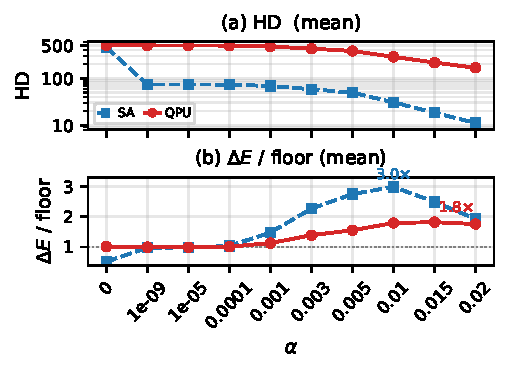
\includegraphics[width=0.99\onecolwid]{figures/fig_sa_vs_qpu.pdf}
\RaggedRight\vskip0.3cm
{\normalsize Same $100$ hardest instances (each $\alpha$: $\ge 91\%$ of reads fail in aggregate). \sacol{Blue}: SA; \qpucol{red}: D-Wave Advantage. \textbf{(a)}~HD (log axis) decreases monotonically yet never reaches $0$. \textbf{(b)}~$\Delta E$ rescaled by each solver's small-$\alpha$ floor onto one axis: both start at $1$; SA rises to a non-monotone $3.0\times$ peak near $\alpha{=}10^{-2}$, the annealer reproducing the same shape more weakly ($1.8\times$).}
\end{block}

\begin{block}{\bnum{8}Table 1 --- Wrong-only means ($\Delta E$ in $\Delta_R$ units)}
\centering\renewcommand{\arraystretch}{1.18}\setlength{\tabcolsep}{8pt}
{\normalsize
\begin{tabular}{l rr rr}
\toprule
 & \multicolumn{2}{c}{\textbf{HD}} & \multicolumn{2}{c}{\boldmath$\Delta E$} \\
\cmidrule(lr){2-3}\cmidrule(lr){4-5}
$\alpha$ & \sacol{SA} & \qpucol{QPU} & \sacol{SA} & \qpucol{QPU} \\
\midrule
$0$            & 458.8 & 501.0 & 0.58 & 24.3 \\
\rowcolor{bandgray}$10^{-9}$      &  73.5 & 499.8 & 1.10 & 23.9 \\
$10^{-5}$      &  73.8 & 498.8 & 1.10 & 23.7 \\
\rowcolor{bandgray}$10^{-4}$      &  73.2 & 497.0 & 1.16 & 24.2 \\
$10^{-3}$      &  68.3 & 474.5 & 1.66 & 27.0 \\
\rowcolor{bandgray}$3\times10^{-3}$ & 58.4 & 427.2 & 2.54 & 33.3 \\
$5\times10^{-3}$ & 49.2 & 380.9 & 3.08 & 37.2 \\
\rowcolor{bandgray}$10^{-2}$      &  30.7 & 285.9 & \hl{3.35} & 42.9 \\
$1.5\times10^{-2}$ & 18.4 & 216.1 & 2.79 & \hl{43.5} \\
\rowcolor{bandgray}$2\times10^{-2}$ & 11.2 & 167.1 & 2.16 & 42.1 \\
\bottomrule
\end{tabular}}
\RaggedRight\vskip0.25cm
{\normalsize Peak $\Delta E$ in \hl{orange}. SA: aggregate failure $\ge 91\%$ at every $\alpha$; QPU: $0\%$ success at every $\alpha$.}
\end{block}

\begin{block}{\bnum{9}Quantum-annealer consistency check}
\RaggedRight
As \textbf{supporting evidence}, a single run of the same $100$ instances on \textbf{D-Wave Advantage} gives $0\%$ success at every $\alpha$. It still shows the \textbf{same pattern}. There is a non-monotone $\Delta E$ peak near $\alpha{=}10^{-2}$ (weaker, $1.8\times$ vs $3.0\times$) and a monotonic HD decrease (\qpucol{$501\to167$}).
\begin{itemize}
  \item Baselines an order of magnitude above SA ($\Delta E\approx 24$ vs.\ $1$) $\Rightarrow$ \textbf{consistent with an instance property, not SA-specific} (one run cannot prove generality).
  \item \lab{Precision floor.} Peak couplers map to Ising $J\approx 0.03$, near the scale where integrated control errors (ICE) matter. We expect a smaller problem scale would push them below ICE and \textbf{flatten the peak}, and leave this to future work.
\end{itemize}
\end{block}

\end{column}
\begin{column}{\sepwid}\end{column}
\end{columns}

%==================================================== FULL-WIDTH CONCLUSION
\vskip0.6cm
\begin{columns}[t]
\begin{column}{\sepwid}\end{column}
\begin{column}{\fullwid}
\begin{block}{\bnum{10}Conclusion}
\RaggedRight\large
Failure-conditioned \sacol{$\Delta E$} is the difficulty diagnostic, and \qpucol{HD} is its complement. The all-sample mean (the success rate) hides the peak. It falls at large $\alpha$ only because more reads succeed, not because the remaining failures are shallower. Whenever an $\alpha$-like hardness parameter is swept, we recommend reporting \textbf{failure-conditioned $\Delta E$ (floor \& peak) together with HD over a fixed set of hardest instances}. The curve persists across SA budgets and is echoed by a supporting quantum-annealer run. So it gives a failure-conditioned diagnostic of the benchmark instances rather than a single difficulty score. Absolute values still depend on the solver and schedule.
\end{block}
\end{column}
\begin{column}{\sepwid}\end{column}
\end{columns}

% ---- footer bar (in-body; full content width) ----
\vskip0.55cm
\begin{columns}[t]
\begin{column}{\sepwid}\end{column}
\begin{column}{\fullwid}
  \begin{beamercolorbox}[wd=\fullwid,sep=0pt,rounded=true]{footbar}
    \hspace{1.3cm}\begin{minipage}[c][1.45cm][c]{\dimexpr\fullwid-2.6cm\relax}
      {\large Code \& instances: \texttt{github.com/YIDEUNKIM/qubo\_dataset}}\hfill{\large\color{accentlight}IEEE QCE 2026 \quad\textbullet\quad Kangwon National University}
    \end{minipage}\hspace{1.3cm}
  \end{beamercolorbox}
\end{column}
\begin{column}{\sepwid}\end{column}
\end{columns}

\end{frame}
\end{document}
